\documentclass[pdftex,12pt,a4paper]{report}

\usepackage[pdftex]{graphicx}
\usepackage[x11names]{xcolor}
\usepackage[explicit]{titlesec}
\usepackage{anysize}
\marginsize{2cm}{2cm}{1cm}{1cm}


\definecolor{black}{RGB}{0,0,0}
\definecolor{grey}{RGB}{90,90,90}
\definecolor{lightgrey}{RGB}{110,110,110}

\newcommand{\HRule}{\rule{\linewidth}{0.5mm}}

\renewcommand{\familydefault}{\sfdefault}

\newcommand{\myItem}[2]{\item \textbf{#1}:#2}


\titleformat{\section}[block]
	{\normalfont\sffamily}
	{
		\colorbox{grey}{\parbox[c][15pt][c]{30pt}{%
		\hfil\color{white}\Large\thesection\hfil}}
	}
	{-6pt}
	{
		\parbox{0.9\linewidth}{%
		\hspace*{0.2em}\color{black}\large\sffamily#1\\[-13pt]\color{grey}\titlerule}
	}
\titlespacing*{\section}{0pt}{3ex plus 1ex minus .2ex}{2ex plus .2ex}

\titleformat{\subsection}[block]
	{\normalfont\sffamily}
	{
		\colorbox{black!50}{\parbox[c][12pt][c]{25pt}{%
		\hfil\color{white}\normalsize\thesubsection\hfil}}
	}
	{-4pt}
	{
		\parbox{0.85\linewidth}{%
		\hspace*{0.4em}\color{black!80}\normalsize\sffamily#1\\[-12pt]\color{black!50}\titlerule}
	}
\titlespacing*{\subsection}{0pt}{3.5ex plus 1ex minus .2ex}{2.3ex plus .2ex}


\titleformat{\chapter}[block]
	{\normalfont\sffamily}
	{
		\begin{flushright}
		\colorbox{black}{\parbox[c][40pt][c]{60pt}{%
		\hfil\color{white}\Huge\thechapter\hfil}}
		\end{flushright}
	}
	{0pt}
	{\parbox{\linewidth}{%
		\vspace*{-5em}\hspace*{0.5em}\color{black}\huge\sffamily#1\\[-25pt]\color{black}
		\titlerule
	}}
\titlespacing*{\chapter}{0pt}{-2cm}{-0.6cm}

\newcommand{\makemytitle}[3] %Args are Title, Subtitle, Author
{
	\begin{titlepage}
	
	\begin{center}
	
	{\colorbox{black!70}{\parbox[c][70pt][c]{200pt}{%
		\color{white}\centering #2}}}
	% Title
	\hrule
	\vspace{1em}
	{\huge\sffamily #1}
	\vspace{1em}
	\hrule 
	\vspace{1em}
	
	#3
	\vfill
	
	
	\end{center}
	
	\end{titlepage}
}



\begin{document}
\makemytitle{Architectural Description Document}
{\LARGE TDT4120 \\ \large Software Architecture}
{{\large\emph{Group X2}}\\[0.2cm]
	Milos Zlatkovic \\
	Dimitry Kongevold \\
	Emil Grunt\\
	Nicolay Thafvelin\\
	Julius Buset Asplin\\
}
\tableofcontents
\chapter{Introduction}
This document contains the architectural decisions related to the quality attributes we have given in the requirements document. We will describe the architectural drivers, stakeholders, architectural views, quality tactics, and the architectural patterns we have chosen.

\chapter{Architectural drivers}
The biggest Architectural Driver in this current project is lack of time. This will affect your architecture to make it more compact and easier to implement.

\section{Modify-ability}
We need to have full Modify-ability regarding new characters, stages, moves and etc. This means that we want to be able to change and add characters, stages and moves and etc without having to change parts of the already written code and without having to concerned about how we write the new code.

Because of the multiple people are working on this project, the modifiability is also and Architectural Driver, the implementation should be “separable“ so we could preside the implementation in a parallel pattern. This also a product of previous driver, short time.

\section{Testability}
We need to be able to test the game all the way through the production so that we can make the right touches to the game so it will be good looking, fun and smooth to play. It is also very crucial for balancing of the characters so that even though they have different moves, they are equally good.

\section{Performance}
The code must be efficient enough so that there wont be any lag or delay while the game is played. We must optimise the calculations and logic and not do more operations than necessary.

\section{Portability}
The game should be playable on both Xbox 360 and computer.

\section{Usability}
The game should be very easy both to start and to play. Their should be easy to find help on which button does what and so on. The objective of the game is quite obvious and therefor needs no introduction.

\chapter{Stakeholders}
\section{Developers}
\begin{itemize}
\item Want a fun playable game as return for their time-investment.
\item Need a good grade on the project, and therefor a good architectural structure.
\end{itemize}

\section{The professor}
\begin{itemize}
\item Wants us to learn about and test/use his advises on architectural structures and program design.
\item Wants us to get a good grade.
\end{itemize}

\section{End user}
\begin{itemize}
\item Wants an easy learned, easy played and fun game.
\end{itemize}

\paragraph{The main concern} is the balance between the number of features and the actual playability of the game. This is also the reason why we want it easy to modify. We will make the standards and the basics of the game finished before adding all the moves and features. We will make it so that adding moves and characters almost only need parameter attributes and pictures to be ready for use.

\chapter{Selection of Architectural Viewpoint}

\section{Logical view}
Logical view shows the Model View Controller architectural pattern. where classes have different functionality. Based on the pattern. the target audience is other architects and stakeholders.

\section{Development view}
The development view describes the static organization of the software in its development environment. You would usually present this in a diagram that presents the different modules/layers of the system.

\section{Scenario view}
Scenario view gives a better understanding over the run time processes and their communications with each other during well known actions in the game. As well as the sequence of the MainGame class and other classes. Target audience is stakeholders as implementation team.

\section{State machine}
The last view is a state machine of the MainGame Window, it explains how the user will navigate himself through the game. Audience is stakeholders.

\chapter{Architectural Tactics}

\section{Modifiability}
To make this project easy to modify we are planning to use Model View Controller architectural pattern, and implement the characters and their moves with only parameter attributes. This makes it easy to change/add characters, maps  or power ups. Model View Controller will also provide grouped implementation, as Character-Controller will only affect the character model. as well as all needed resources needed for Draw method will be allocated under model. were it’s easy to check for consistences.

\section{Testability}
We are going to start out very simple, so that the testing, as in playing the game, can start early. Since we are doing it this way, we wont need the computer to perform actual tests for the most part. We can test it simply by building the project and start testing it manually.

To test the individual methods and the logic itself we will try to separate logic from data and GUI, which will make testing of them easier.

\section{Performance}
We will do performance testing to weed out resource hogs, and find out which methods use the most computational power and alter or remove them.

\section{Portability}
We will only use classes which are supported by Xbox 360, and surround any platform specific code with compiler pragma to avoid duplication of code.

\section{Usability}
This has nothing to do with the architecture.

\chapter{Architectural Patterns}
These are the architectural patterns we're planing to use 
\section{MVC - Model, View and Controller}
We chose Model View Controller architectural pattern because it gave us the best modifiability  as well as it separates code into small fragments that are easy to test and distribute the work load through the group.

\section{SOA - Service Oriented Architecture}
The Game class in the XNA Framework provides an infrastructure for registering and providing application level services. By grouping related functionality into classes and offering them as “services” specified through an interface, the functionality can be provided without compromising modifiability.

\section{Observer pattern}
The communication within the game will primarily be through firing of events and registration of callbacks. This will improve the modifiability a lot. We also will use state pattern in the characters and the map class.

\chapter{Views}
\section{Logical Views}
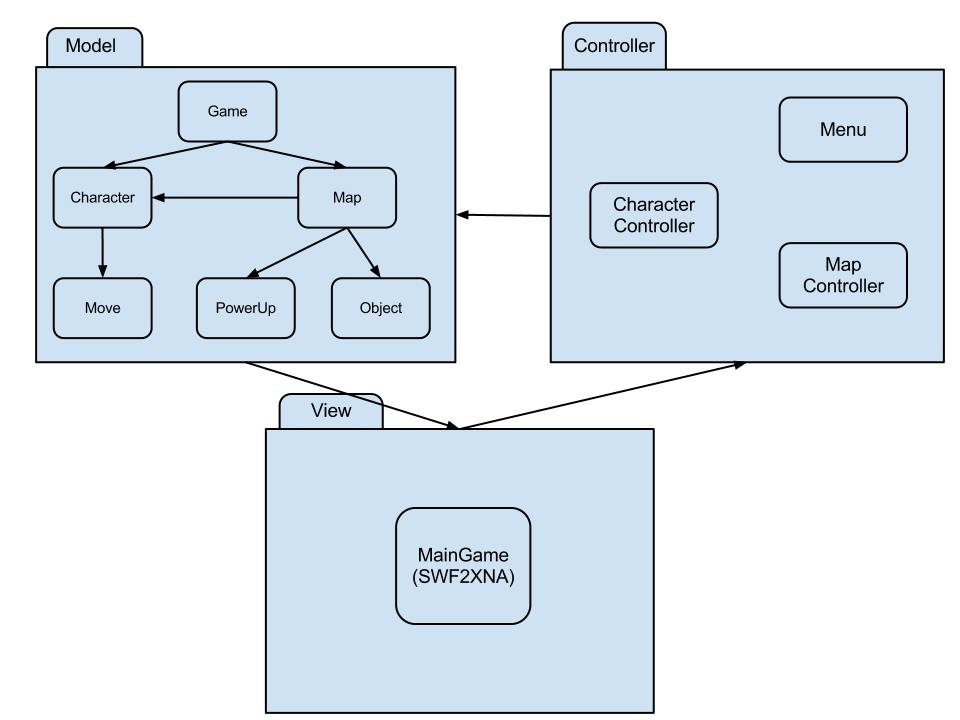
\includegraphics[scale=0.45]{logical.jpg}

%\section{Development view}

\section{Scenario view}
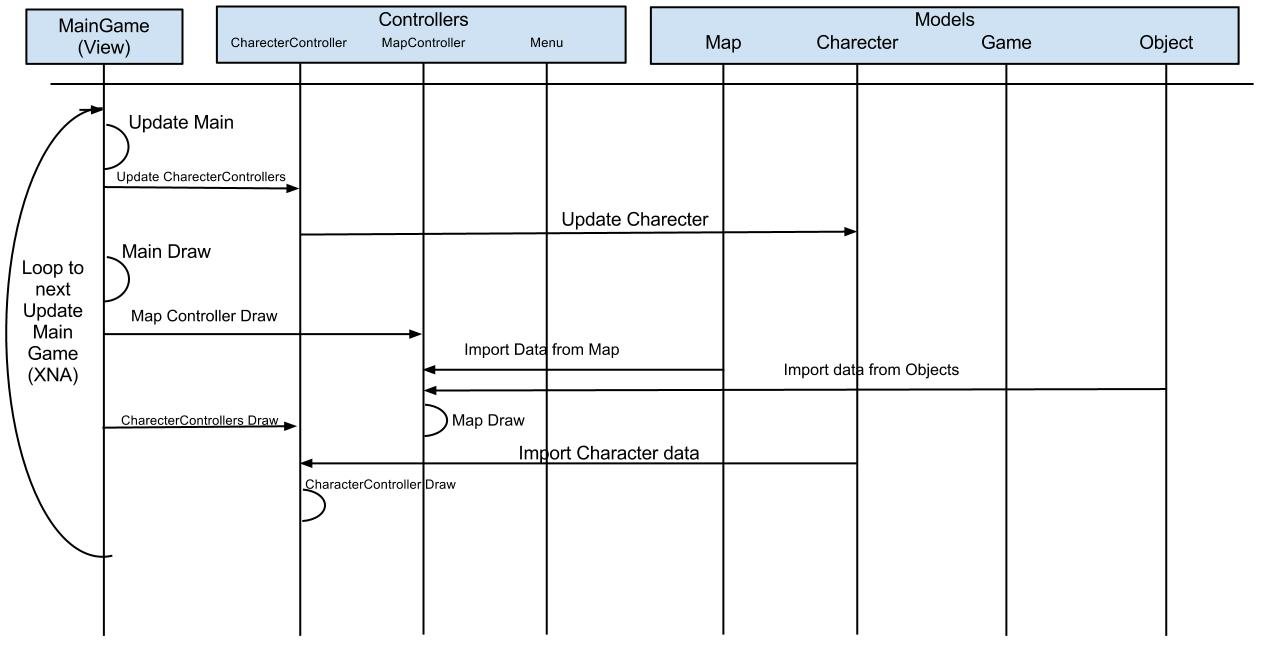
\includegraphics[scale=0.4]{Seq.jpg}

\section{State machine}
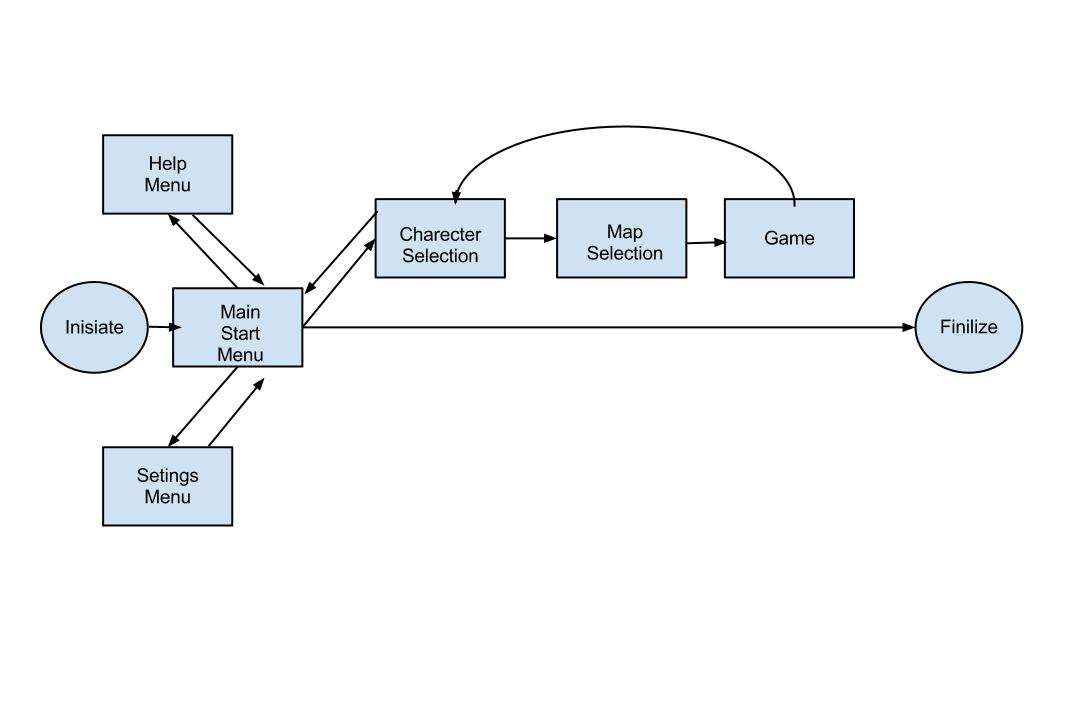
\includegraphics[scale=0.45]{State.jpg}

\chapter{References}
This is the references we used to complete this document 
\section{Books}
\begin{itemize}
\item "Software Architecture in Practice, Second Edition", Len Bass, Paul Clements, Rick Kazman, Addision-Wesley, 2003, ISBN 0-321-15495-9
\item "Game Architecture and Design - A New Edition", Andrew Rollings and Dave Morris
\end{itemize}

\section{Webpages}
\begin{itemize}
\item http://en.wikipedia.org/wiki/SOA
\item http://en.wikipedia.org/wiki/Model–view–controller
\item http://en.wikipedia.org/wiki/Observer\_pattern
\end{itemize}

\end{document}